
The flow past a moving flat plate is one of the few cases for which analytical solutions work well with heuristic model of vortex shedding.
Following the work by Theodore Theodorsen, we analyze the flow past a flat plate with both heaving and small-angle pitching motion. 
Further, we find the optimal stroke for maximum energy extraction from the ambient flow, and try to uncover the mechanism behind the selection of optimal frequency. 

\begin{figure}
 \centering
 \noindent \\
 \begin{tikzpicture}[scale=3.5]
 
  \draw[dashed] (-1, 0) -- (1, 0);
 \draw[very thick] (150:1cm) -- (-30:1cm);
 \draw[<-,thick] (150:0.25cm) arc (150:180:0.25cm);
   \node at (165:0.4cm) {$\dot{\alpha}$};
\draw[->,thick] (0, 0.1) -- (0, 0.4);
  \node at (0.1,0.25) {$\dot{h}$};
 \foreach \y in {-0.6, -0.3, 0, 0.3, 0.6}
   \draw[->, thick] (-2.5, \y cm) -- (-1.5, \y cm);
 \node at (-2, 0.7) {$\Uinf$};
 
 \end{tikzpicture}

\caption{A schematic of flow past a flat plate with pitching and heaving.}
\label{fig:FlatPlate}
\end{figure}


\section{Flow past a flat plate}

The flow around a flat plate can be decomposed into two parts: noncirculatory flow, and circulatory flow induced by shed vortices.
With those, the forces and moments acting on the plate, and then the total work done by the fluid on the plate, are calculated.

\subsection{Noncirculatory flow}

In this part, the velocity (potential) which satisfies the Laplace equation with the no-penetration boundary condition is calculated.
The general idea is to transform the problem of flow past a flat plate in one space into that of flow past a circle in another space, which is readily solved. 
The line geometry of a flat plate with length $2b$ in $z$-plane can be obtained from a circle with radius $b$ in $\zeta$-plane, through the Zhukovsky conformal mapping
\begin{align} \label{eqn:ConformalMapping}
2z = \zeta + \frac{b^2}{\zeta},    \text{   or inversely~~~~~}   \zeta =z \pm \sqrt{z^2-b^2}.
\end{align}
Note that we have an extra factor $2$ in front of $z$ compared with the traditional transformation and by this the plate is simply the geometric projection of the circle on the  $x$ axis.
However, this transformation with factor $2$ doesn't preserve the velocity at infinity and when we transform the flow back into that in $z$-plane, the free stream velocity at infinity should be reduced by half.

\begin{figure}
 \centering
 \noindent \\
 \begin{tikzpicture}[scale=2]

\foreach \x in {2}
{
 \draw[->] (-1.25-\x,0) -- (1.25-\x,0) node[right] {$Re(\zeta)$};
 \draw[->] (-\x,-1.25) -- (-\x,1.25) node[above] {$Im(\zeta)$};
 \node at (-\x+0.2, -0.2) {$O$};
 \draw[very thick,blue] (-\x,0) circle (1cm);
 \draw[->] (-\x, 0) -- ++(30:1);
 \node at (-\x+0.4,0.4) {$b$};
 \node at (-1-\x,1) {$\zeta-plane$};
 
 \draw[->] (-1.25+\x,0) -- (1.25+\x,0) node[right] {$Re(z)$};
 \draw[->] (\x,-1.25) -- (\x,1.25) node[above] {$Im(z)$};
 \node at (\x+0.2, -0.2) {$O$};
 \draw[very thick,blue] (-1+\x,0) -- (1+\x,0);
 \node at (-1+\x,0.2) {$-b$};
 \node at (1+\x,0.2) {$b$};
 \node at (-1+\x,1) {$z-plane$}; 
}
 
 \node at (0.3, 0) {$\Longleftrightarrow$};
 
 \end{tikzpicture}

\caption{The Zhukovsky's conformal mapping between a circle and a line.}
\label{fig:ConformalMapping}
\end{figure}

As we know, the potential flow around a 2D circular cylinder with radius $b$ placed in an otherwise uniform free stream $(U,V)$ is the superposition of the free stream and the flow due to a dipole, with the complex potential
\begin{align}
w(\zeta) = (U-iV)\zeta+\frac{(U+iV)b^2}{\zeta}.
\end{align} 
Plugging the Zhukovsky mapping in (remember to reduce the free stream velocity by half), we get the complex potential around the flat plate in the $z$-plane as
\begin{align}
w(z) = Uz \mp iV\sqrt{z^2-b^2}.
\end{align} 
For the calculation of the forces and moments on the plate, we only need the flow quantities evaluated on the surface of the plate.
Let $z = bx$ with $x \in [-1, 1]$, and we get the potential (real part of complex potential) as
\begin{align}
\phi(x) = Ubx \pm Vb\sqrt{1-x^2},
\end{align} 
where, the plus and minus signs correspond to the upper and lower surfaces of the plate respectively. 
The first term $Ubx$ is the free stream, and in the following, potential $\phi$ will only refer to the second term, which is the perturbation to the free stream (on the upper surface of the plate)
\begin{align}
\phi(x) = Vb\sqrt{1-x^2}.
\end{align} 
Apply the equation above to the flat plate, lying with a small fixed angle $\alpha$ (clockwise is positive) relative to the free stream $U$ and moving vertically with speed $\dot{h}$ (upward is positive).
Relative to the plate, the free stream is approximately $(U, U \alpha - \dot{h}))$ and thus the corresponding potential is
\begin{align}
\phi(x) = (U \alpha - \dot{h}) b \sqrt{1-x^2}.
\end{align} 
However, if $\alpha$ is not a constant, we have another contribution from the rotation $\dot{\alpha}bx$ of the plate, which can be obtained by the superposition of flow due to the motion of each infinitesimal element of the plate.
This contribution turns out to be $\phi(x) = \frac{1}{2}\dot{\alpha}xb^2\sqrt{1-x^2}$, and so the total potential of noncirculatory flow (except the free stream) is
\begin{align}
\phi_{nc}(x) = (U\alpha - \dot{h} + \frac{1}{2}\dot{\alpha}bx) b\sqrt{1-x^2}.
\end{align} 

With the velocity potential, we are able to calculate the local pressures and by integration to obtain the total forces and moments on the plate.
Employing the Bernoulli's equation for unsteady flow, the local pressure is, except for a constant,
\begin{align}
p = -\rho (\frac{\partial \phi}{\partial t} + \frac{q^2}{2}),
\end{align} 
where the local velocity is $q = U + \frac{\partial \phi}{\partial (bx)}$.
Then we obtain the pressure difference between lower and upper surfaces (lower surface has potential $-\phi$) at $x$ as
\begin{align}
p(x) = 2 \rho [\frac{\partial \phi}{\partial t} + U\frac{\partial \phi}{\partial (bx)}].
\end{align} 
Finally, we are able to write down the total forces (upward is positive) and moments (anti-clockwise is positive) acting on the plate due to noncirculatory part of the flow as
\begin{align}
P_{nc} & = \int^{1}_{-1} p(x)bdx
   = \pi\rho b^2(U\dot{\alpha} - \ddot{h}),   \\
M_{nc} & = \int^{1}_{-1} p(x)b^2xdx
   = \pi\rho b^2[\frac{1}{8}b^2\ddot{\alpha} - U(U\alpha - \dot{h})].
\end{align}


\subsection{Circulatory flow}

In order to (partially) account for the viscous effect, we assume certain vorticity is shed from the plate and forms a thin layer of vortex sheet, extending from the trailing edge of the plate to infinity, and the exact amount of the shed vorticity will be determined in the next section.
In this part, we shall calculate the contribution from the flow induced by this vortex sheet kinematically.
The general approach is the same as that for noncirculatory flow, transforming the problem of flow past a flat plate to that of flow past a circle.

\begin{figure}
 \centering
 \noindent \\
 \begin{tikzpicture}[scale=2]

\draw[dashed] (-1.25, 0) -- (4, 0);
\draw[very thick, blue] (0, 0) circle (1);
\node at (0, 0.1) {$O$};
\draw[->, thick] (0, 0) -- (215:1);
\node at (205:0.5) {$1$};
\foreach \x in {3}
{
 \draw[->, thick] ($(\x, 0)+(-135:0.1)$) arc (-135:135:0.1);
 \node at (\x+0.2, 0.2) {$\Gamma$};
 \node at (\x+0.2, -0.3) {$(X_0, 0)$};
 \draw[<-, thick, red] ($(1/\x, 0)+(45:0.1)$) arc (45:315:0.1);
 \node at (1/\x+0.2, 0.2) {$-\Gamma$};
 \node at (1/\x+0.2, -0.3) {$(1/X_0, 0)$};
}
 
 \end{tikzpicture}

\caption[The flow induced by a point vortex outside a circle through image method]{The flow induced by a point vortex outside a circle through image method: the flow induced by a vortex $\Gamma$ outside a circle $(X_0, 0)$ and with no normal velocity on surface of circle is the same as the superposition of the flow induced by two vortices in free space: the original vortex and its image vortex $-\Gamma$ at $(1/X_0, 0)$.}
\label{fig:ImageMethod}
\end{figure}

As we know, the flow around a circle (with radius 1) due to a vortex element $d\Gamma$ (anti-clockwise is positive) at $(X_0, 0)$ ($X_0 > 1$) can be obtained through the image method (shown in Figure \ref{ref:ImageMethod}) by the superposition of the flow due to this vortex and an image vortex $-d\Gamma$ at $(1/X_0,0)$ as
\begin{align}
\mathrm{d}\phi_\Gamma (X,Y; X_0) & = \frac{\mathrm{d}\Gamma}{2\pi}[\arctan \frac{Y}{X-X_0} - \arctan \frac{Y}{X-1/X_0}]  \\
            & =  \frac{\mathrm{d}\Gamma}{2\pi}\arctan \frac{(X_0-1/X_0)Y}{X^2-(X_0+1/X_0)X+Y^2+1}.
\end{align}
On the (upper half) circle with $X = x$ and $Y = \sqrt{1-x^2}$, the equation above can be written as
\begin{align}
\mathrm{d}\phi_\Gamma (X = x,Y = \sqrt{1-x^2}; X_0)  =  \frac{\mathrm{d}\Gamma}{2\pi}\arctan \frac{(X_0-1/X_0)\sqrt{1-x^2}}{2-(X_0+1/X_0)x}.
\end{align}
Transforming to the space of the plate through the Zhukovsky conformal mapping defined earlier in \eqref{eqn:ConformalMapping}, the field point $(x, \sqrt{1-x^2})$ maps to $(x, 0)$ and the vortex position $(X_0, 0)$ maps to $(x_0, 0)$ with $X_0 + 1/X_0 = 2x_0$ or $X_0 = x_0 + \sqrt{x_0^2-1}$.
With these, we can write down the potential at $x$ on the upper surface of a flat plate due to vortex element $d\Gamma$ at $(x_0, 0)$ as
\begin{align}
\mathrm{d}\phi (x; x_0) = \frac{\mathrm{d}\Gamma}{2\pi} \arctan \frac{\sqrt{1-x^2}\sqrt{x_0^2-1}}{1-x_0x}.
\end{align}
Similarly, on the lower surface of the plate the potential is $-\phi(x; x_0)$.

For the pressure difference between lower and upper surfaces, we have the same relation $p = 2 \rho[\frac{\partial \phi}{\partial t} + U\frac{\partial \phi}{\partial (bx)}]$.
But since the vortex elements are regarded as moving to the right relative to the plate with the free stream velocity $U$,  we have $\frac{\partial \phi}{\partial t} = U\frac{\partial \phi}{\partial (bx_0)}$ and so 
\begin{align}
p & = 2\rho U [\frac{\partial \phi}{\partial (bx_0)} + \frac{\partial \phi}{\partial (bx)}]  \\
   & =  \frac{\rho U \mathrm{d}\Gamma}{\pi b} \frac{x_0+x}{\sqrt{1-x^2}\sqrt{x_0^2-1}}.
\end{align}
By integration over all the vortex elements with distribution on a line $d\Gamma(x_0) = \kappa(x_0)bdx_0$, we get the distribution of potential and pressure difference on the plate with respect to the line vortex density $\kappa(x_0)$ as follows,
\begin{align}
\phi_c(x) & =  \frac{b}{2\pi} \int_{1}^{\infty}\arctan \frac{\sqrt{1-x^2}\sqrt{x_0^2-1}}{1-x_0x} \kappa(x_0) \mathrm{d}x_0, \\
p_c(x) &  =  \frac{\rho U}{\pi} \int_{1}^{\infty}\frac{x_0+x}{\sqrt{1-x^2}\sqrt{x_0^2-1}} \kappa(x_0) \mathrm{d}x_0.
\end{align}
With further integration over the plate, the total forces (upward is positive) and moments (anti-clockwise is positive) acting on the plate due to the circulatory flow are obtained as
\begin{align}
P_c & =  \int_{-1}^{1} p_c (x) b \mathrm{d}x
   =  \rho U b \int_{1}^{\infty} \frac{x_0}{\sqrt{x_0^2-1}} \kappa(x_0) \mathrm{d}x_0, \\
M_c & =  \int_{-1}^{1} p_c (x) b^2 x \mathrm{d}x
   =   \frac{1}{2} \rho U b^2 \int_{1}^{\infty} \frac{1}{\sqrt{x_0^2-1}} \kappa(x_0) \mathrm{d}x_0.
\end{align}
Note that since the vortex element is considered stationary with respect to the fluid elements, we have $\kappa (x_0) = f(Ut - x_0)$, where $t$ is the time since the beginning of the motion and $Ut-x_0$ is the distance from the location of the first vortex element.


\subsection{Magnitude of circulation}

In this section, the magnitude of the circulation is determined by the classical Kutta condition, which requires that no infinite velocities exist at the trailing edge of the plate, or at $x = 1$,
\begin{align}
\frac{\partial (\phi_{nc} + \phi_c)}{\partial x} = \text{finite}.
\end{align}
Plug in the expressions for $\phi_{nc}$ and $\phi_c$ from the previous two sections and some rearranging gives the following relation
\begin{align}       \label{eqn:Kutta}
\frac{1}{2\pi} \int_{1}^{\infty} \sqrt{\frac{x_0+1}{x_0-1}} \kappa(x_0) \mathrm{d}x_0 = U \alpha - \dot{h} + \frac{1}{2}b\dot{\alpha}.
\end{align}

\begin{figure}
\begin{center}
 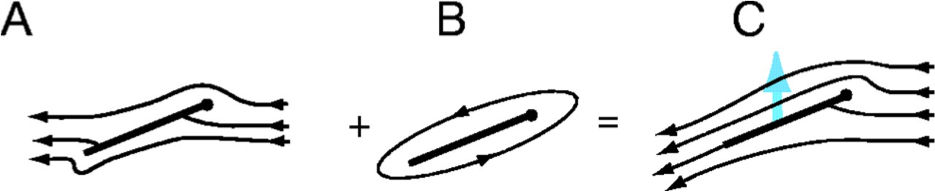
\includegraphics[width=14cm]{Figures/theodorsen/KuttaCondition.png}
\end{center}
\caption[Schematic of Kutta condition]{Schematic of how Kutta condition works. (A) shows the potential flow without any circulation around the plate and the flow goes around the sharp edge of the plate with a singular point of infinite pressure. By adding proper amount of circulation (B) to the flow, the flow leaves the trailing edge of the plate smoothly (C) and the singularity there is removed.}
\label{fig:KuttaCondition}
\end{figure}

For our purpose, the parameters of stroke on the right hand side of (\eqref{eqn:Kutta}), say $\alpha$ and $\dot{h}$, are given and the expression above determines the circulation function $\kappa(x_0)$ , and further the flow around the plate. 
In the following, we will write the oscillating parameter as
\begin{align}
Q \equiv U \alpha - \dot{h} + \frac{1}{2}b\dot{\alpha},
\end{align}
and further introduce the function
\begin{align}
C \equiv \frac{\int_{1}^{\infty} \frac{x_0}{\sqrt{x_0^2-1}} \kappa(x_0) \mathrm{d}x_0}{\int_{1}^{\infty} \frac{x_0+1}{\sqrt{x_0^2-1}} \kappa(x_0) \mathrm{d}x_0},
\end{align}
which is the deficiency factor representing effects of vorticity shedding from the trailing edge and generally depends on the oscillating parameters of the plate through (\ref{eqn:Kutta}), especially the oscillating frequency.
With these definitions, the force and moment acting on the plate due to the circulatory flow can be rewritten as
\begin{align}
P_c & = 2\pi \rho b U Q C,  \\
M_c & = \pi \rho b^2 U Q (1 - C).
\end{align}

\subsection{Theodorsen's function C}

If the plate oscillates periodically, that is, the stroke parameters $\alpha$ and $h$ are both periodic functions of time with a single mode, we can write the circulation distribution as
\begin{align}
\kappa(x_0) = \kappa_0 \exp \{i[k(\frac{s}{b}-x_0)+ \varphi] \},
\end{align}
where $s = Ut$ denotes the distance from the first vortex element to the plate, and $k$ is the dimensionless wavenumber.
For the special case of harmonic oscillation, we don't need to calculate the magnitude $\kappa_0$ explicitly through the relation (\ref{eqn:Kutta}), because it will cancel out and not appear in the expression of $C$ as
\begin{align}
C(k) = \frac{\int_{1}^{\infty} \frac{x_0}{\sqrt{x_0^2-1}} e^{-ikx_0} \mathrm{d}x_0}{\int_{1}^{\infty} \frac{x_0+1}{\sqrt{x_0^2-1}} e^{-ikx_0} \mathrm{d}x_0}.
\end{align}
The integrals on the numerator and denominator can both be expressed using Bessel functions, and then the equation can be written as
\begin{align}
C(k) & =  \frac{\frac{\pi}{2}(-J_1+iY_1)}{\frac{\pi}{2}[-(J_1+Y_0)+i(Y_1-J_0)]}
          \equiv  F(k) + iG(k),
\end{align}
with the real and imaginary part being
\begin{align}
F & = \frac{J_1(J_1+Y_0)+Y_1(Y_1-J_0)}{(J_1+Y_0)^2+(Y_1-J_0)^2},  \\
G & = -\frac{Y_1Y_0+J_1J_0}{(J_1+Y_0)^2+(Y_1-J_0)^2}.
\end{align}
For general motions of the plate, we can write $Q$  and $\kappa$ as the superposition of different modes by Fourier transform and then relate the magnitude of each mode through relation (\ref{eqn:Kutta}). In that case, the magnitude of each mode of the circulation will explicitly appear in the expression of $C(k)$.
$C(k)$ is of fundamental importance in this model of oscillating plate and its real and imaginary parts are plotted in Figure

\begin{figure}
 \centering
 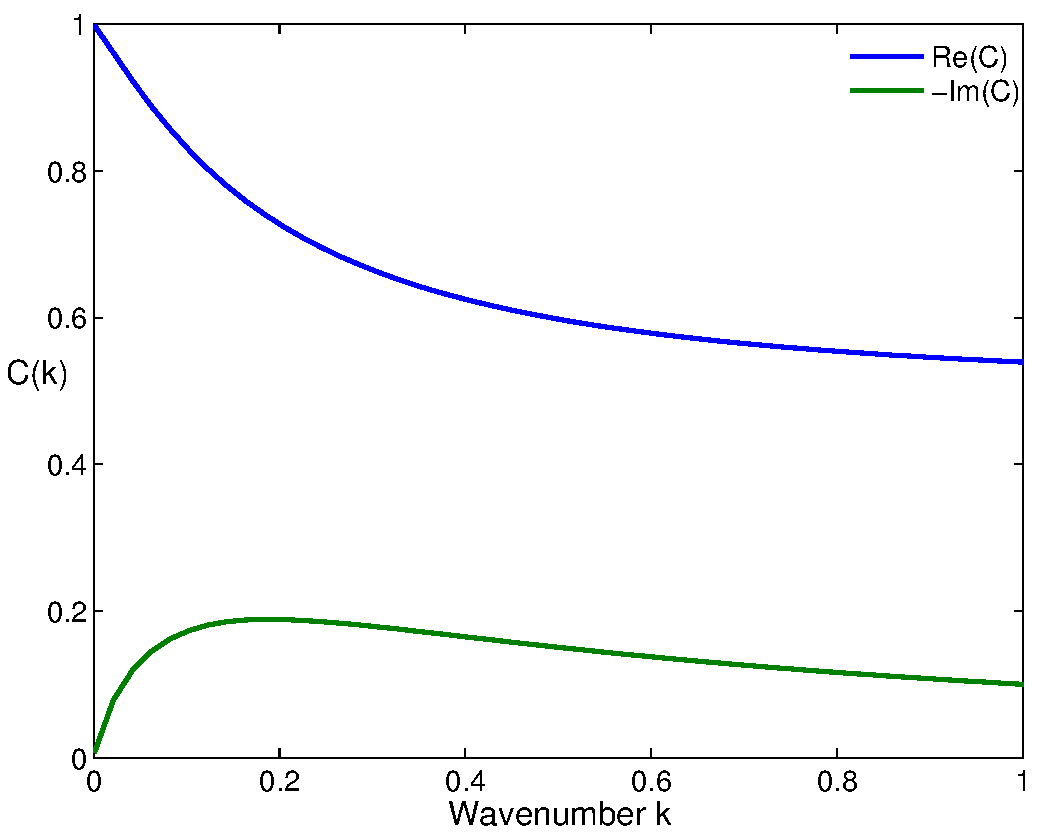
\includegraphics[width=10cm]{Figures/theodorsen/TheodorsenFunction.pdf}
\caption{Theodorsen's function with respect to the wavenumber}
\label{fig:TheodorsenFunction}
\end{figure}


\section{Optimal frequency for energy extraction}

In this part, we will investigate the dependence of energy extraction efficiency on the oscillating strokes of plate and try to find the optimal frequency.
For simplicity, we will still look at the oscillating plate with a harmonic motion, that is,
\begin{align}
\alpha = Re(\alpha_0 e^{i\omega t}),    \text{    and   }        h = Re(b h_0 e^{i\omega t}),
\end{align}
with the complex amplitudes $\alpha_0$ and $h_0$ dimensionless.

\subsection{Energy extraction}

First, we can easily see that the average work done by the noncirculatory flow on the plate over one period is zero. 
The work rate is
\begin{align}
W_{nc} & =  P_{nc} \dot{h} - M_{nc} \dot{\alpha}  \\
       & =  \pi \rho b^2 (U^2 \alpha \dot{\alpha} - \frac{1}{8} b^2 \dot{\alpha} \ddot{\alpha} - \dot{h} \ddot{h})  \\
       & =  \pi \rho b^2 \frac{1}{2} \frac{d}{dt} (U^2 {\alpha}^2 - \frac{1}{8} b^2 {\dot{\alpha}}^2 - {\dot{h}}^2 ),
\end{align}
and the corresponding average value vanishes obviously as follows
\begin{align}
<W_{nc}> = \frac{\omega}{2\pi} \int_{0}^{2\pi/\omega} W_{nc} \mathrm{d}t = 0.
\end{align}
Then the work done by the circulatory flow is
\begin{align}
W_{c}   = & P_{c} \dot{h} - M_{c} \dot{\alpha}  \\
         = & 2\pi \rho b U Re(CQ) Re(i \omega bh_0 e^{i\omega t}) - \pi \rho b^2 U Re( (1 - C)Q ) Re( i \omega \alpha_0 e^{i\omega t} )  \\
     = & 2\pi \rho b U \frac{1}{4} [ C(U\alpha_0 - i \omega bh_0 + \frac{1}{2} i \omega b\alpha_0) i \omega bh_0 e^{i2\omega t} + c.c. \\
       &  + C(U \alpha_0 - i \omega bh_0 + \frac{1}{2} i\omega b\alpha_0) (-i \omega b h_0^{*}) + c.c.]  \\
       &  - \pi \rho b^2 U \frac{1}{4} [ (1 - C) (U \alpha_0 - i \omega b h_0 + \frac{1}{2} i\omega b\alpha) i\omega \alpha_0 e^{i2\omega t} + c.c. \\
       &   + (1 - C) (U \alpha_0 - i \omega bh_0 + \frac{1}{2} i\omega b\alpha_0) (-i\omega \alpha_0^{*}) + c.c.].
\end{align}
Averaging over one period, noticing that the first and third line have no contributions, gives 
\begin{align}
<W_{c}>  = & \frac{1}{2} \pi \rho b U [C(U \alpha_0 - i \omega bh_0 + \frac{1}{2} i\omega b \alpha_0) (-i \omega b h_0^{*}) + c.c.]     \\
                                  & - \frac{1}{4} \pi \rho b^2 U [(1 - C) (U \alpha_0 - i \omega bh_0 + \frac{1}{2} i\omega b\alpha_0) (-i\omega \alpha_0^{*}) + c.c.]
\end{align}
which can be rewritten with standard quadratic form (with $\omega = Uk/b$) as
\begin{align}
<W_{c}(k)>  = \frac{1}{4}{\pi \rho U^3 b} X^* M(k) X,
\end{align}
with
\begin{align}
X =  \begin{bmatrix} h_0  \\  \alpha_0   \end{bmatrix},
M(k) = \begin{bmatrix}   -4k^2 F   &  (2kG+k^2) - i(2kF - 2k^2G)  \\
                         (2kG+k^2) + i(2kF - 2k^2G)  &   2kG - k^2(1 - F)  \end{bmatrix}.
\end{align}

\subsection{Optimal stroke}

Our goal here is to maximize $X^* M X$ under the constraint $X^* X = 1$.
It is readily shown as follows that this is equivalent to find the maximum eigenvalue of $M$.
The objective function with Lagrangian multiplier is 
\begin{align}
f(X; \lambda) = X^* M X - \lambda (X^* X - 1),
\end{align}
and setting the derivative as zero gives $MX = \lambda X$ and the corresponding extreme value of $f$ is found to be $\lambda$.

For different wavenumber $k$, the corresponding optimal energy efficiency is numerically computed as the larger eigenvalue of $M$ and plotted in Figure \ref{fig:Theodorsen}, in which the corresponding phase difference between pitching and heaving is also shown.
The figure clearly shows two different asymptotes for small and large wavenumber (frequency) $k$ respectively, and the optimal wavenumber $k$ can be located somewhere in between.
For small wavenumber, the energy efficiency is generally very low and grows linearly with the wavenumber, and the optimal stroke has a large phase difference between heaving and pitching.
For the case of large wavenumber, the optimal stroke has almost no phase lag between pitching and heaving, and the energy coefficient tends to a constant.
These two different asymptotic behaviors can be verified by the asymptotic behaviors of the matrix $M$ later.
More importantly, the optimal wavenumber can be located in between with the reduced frequency $f = k/\pi = 0.2$ (we have different scales of nondimensionalization than those used typically), which is very close to the value $0.15$ found by Zhu through parameter sweeping with direct numerical simulations.

\begin{figure}
\begin{center}
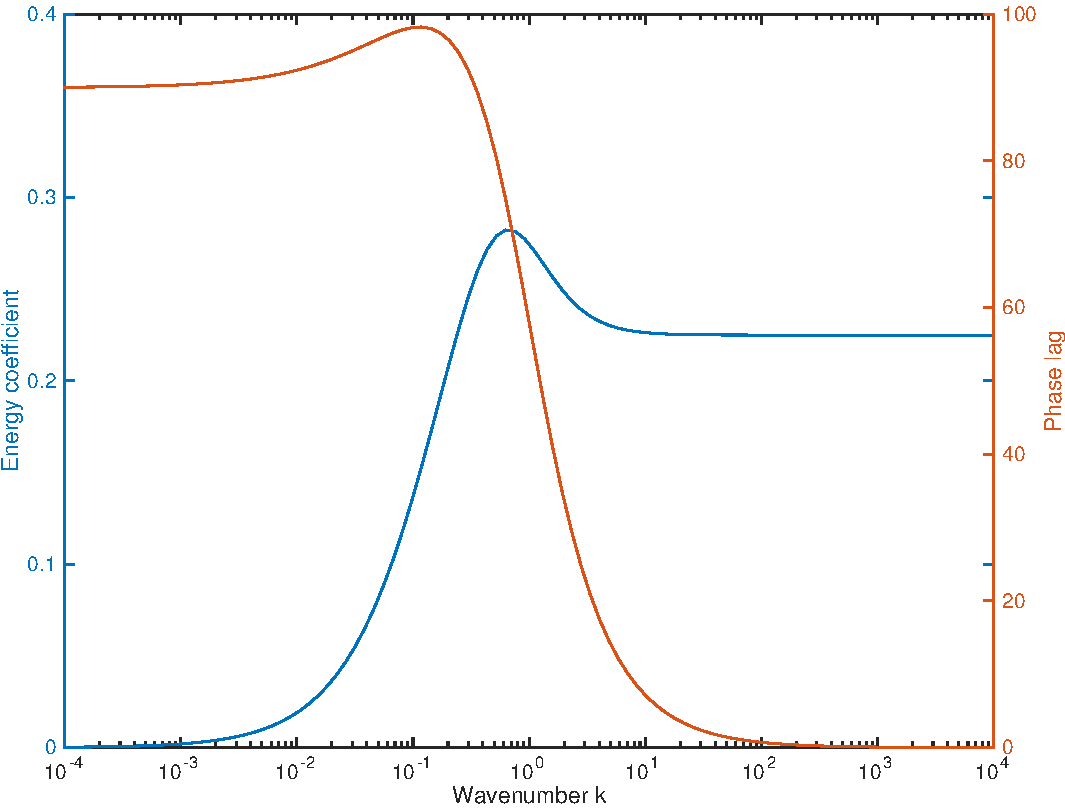
\includegraphics[width=13cm]{Figures/theodorsen/TheodorsenEnergy.pdf}
\end{center}
\caption[The optimal stoke for energy extraction at different oscillating frequencies of plate]{The optimal energy coefficient for different oscillating frequencies is shown, along with the phase lag between the corresponding pitching and heaving motion. Two different asymptotic behaviors are captured. For small wavenumber, the optimal stroke has large phase difference between heaving and pitching motions, and the energy efficiency, which grows linearly with the wavenumber, is generally very low. For large wavenumber, the phase difference between the corresponding heaving and pitching motion is small, and the energy coefficient goes to a constant value. In between, the optimal frequency for energy extraction can be located, and the corresponding phase difference is relatively large, around $70^0$.}
\label{fig:Theodorsen}
\end{figure}

In the following, we can verify the two different asymptotic behaviors observed in Figure \ref{fig:Theodorsen} through asymptotic analysis of matrix $M$.
For small $x$, the Bessel's functions have the following asymtotes
\begin{align}
Y_0(x)  \simeq  \frac{2}{\pi} \ln x,  \hspace{3mm} 
Y_1(x)  \simeq  -\frac{2}{\pi x}, \hspace{3mm}
J_0(x) \simeq 1, \hspace{3mm}
J_1(x) \simeq \frac{x}{2},
\end{align}
and accordingly
\begin{align}
F(k) \simeq 1,  \hspace{30pt}   G(k) \simeq k \ln k
\end{align}
and
\begin{align}
M \simeq \begin{bmatrix} 
-4k^2   &  2k^2 \ln k - i2k  \\
2k^2 \ln k + i2k  &   2k^2 \ln k 
\end{bmatrix}.
\end{align}
With these approximations, the maximum eigenvalue and the corresponding eigenvector are found to be
\begin{align}
\lambda_{max} \simeq 2k,   \hspace{1cm}
X \simeq   \frac{1}{\sqrt{2}}
\begin{bmatrix} k \ln k - i \\  1   \end{bmatrix}.
\end{align}
We see that in this low-frequency regime the optimal stroke has a phase difference $\phi$ between pitching and hitching, which tends to $90^o$ as $k$ goes to 0, and the corresponding optimal energy coefficient is linearly proportional to the frequency, consistent as the numerical data shown in Figure \ref{fig:Theodorsen}.

For large $x$, the Bessel's functions have different behaviors from the case of small $x$ as
\begin{align}
Y_0(x) & \simeq  \sqrt{\frac{2}{\pi x}} [ \sin (x-\frac{\pi}{4}) - \frac{1}{8x} \cos (x - \frac{\pi}{4}) ], \\
Y_1(x) & \simeq  \sqrt{\frac{2}{\pi x}} \large{[} -\cos (x-\frac{\pi}{4})+\frac{3}{8x} \cos (x - \frac{\pi}{4}) \large{]}, \\
J_0(x) & \simeq  \sqrt{\frac{2}{\pi x}} \large{[} \cos (x-\frac{\pi}{4}) + \frac{1}{8x} \sin (x - \frac{\pi}{4}) \large{]}, \\
J_1(x) & \simeq  \sqrt{\frac{2}{\pi x}} \large{[} \sin (x-\frac{\pi}{4}) + \frac{3}{8x} \cos (x - \frac{\pi}{4}) \large{]},
\end{align}
and accordingly
\begin{align}
F(k) \simeq \frac{1}{2},   \hspace{25pt}  G(k) \simeq -\frac{1}{8k}
\end{align}
and
\begin{align}
M \simeq \begin{bmatrix}   -2k^2   &  (k^2 - \frac{1}{4}) - i\frac{5}{4}k  \\
                        (k^2 - \frac{1}{4}) + i\frac{5}{4}k &   -\frac{1}{2}k^2 - \frac{1}{4}  \end{bmatrix}.
\end{align}
In this case, the maximum eigenvalue and the corresponding eigenvector are found to be
\begin{align}
\lambda_{max} = \frac{9}{40} + O(\frac{1}{k^2}), \hspace{1cm}
X \simeq \frac{2}{\sqrt{5}}
\begin{bmatrix} \frac{1}{2} - i \frac{5}{8k}   \\     1     \end{bmatrix}.
\end{align}
We see that in this high-frequency regime the maximum efficiency of energy extraction tends to a constant as the frequency grows, and the corresponding optimal stroke has almost no phase difference between pitching and heaving motions.

For comparison, our results are also displayed along with experimental data from both flume and field in Figure \ref{fig:Strouhal}.
For the purpose of high energy coefficient, the pitching is chosen with a large amplitude $\alpha_0 = 70^o$, three different heaving amplitudes $h_0 = [2, 2.5, 3]b$ are looked at, and the phase difference between heaving and pitching is chosen large as $\phi = 90^o$.
Note that we use slightly different scales for nondimensionalization than those typically used by other researchers.
For consistency of comparison, the energy efficiency $\eta$ is defined as the portion of flow energy flux within the swept area extracted by the plate, i.e. $\eta = \overline{W} / \frac{1}{2} \rho U^3 Y_p$, where $Y_p$ is calculated as the difference between the highest and lowest vertical positions reached by the leading/trailing edges, and the reduced frequency is scaled as $f = k/\pi$ instead of our wavenumber $k$.
Figure \ref{fig:Strouhal} shows great agreement on the general trends of energy efficiency, although some quantitative discrepancies exist among them.

\begin{figure}
\begin{center}
\begin{tabular}{c}
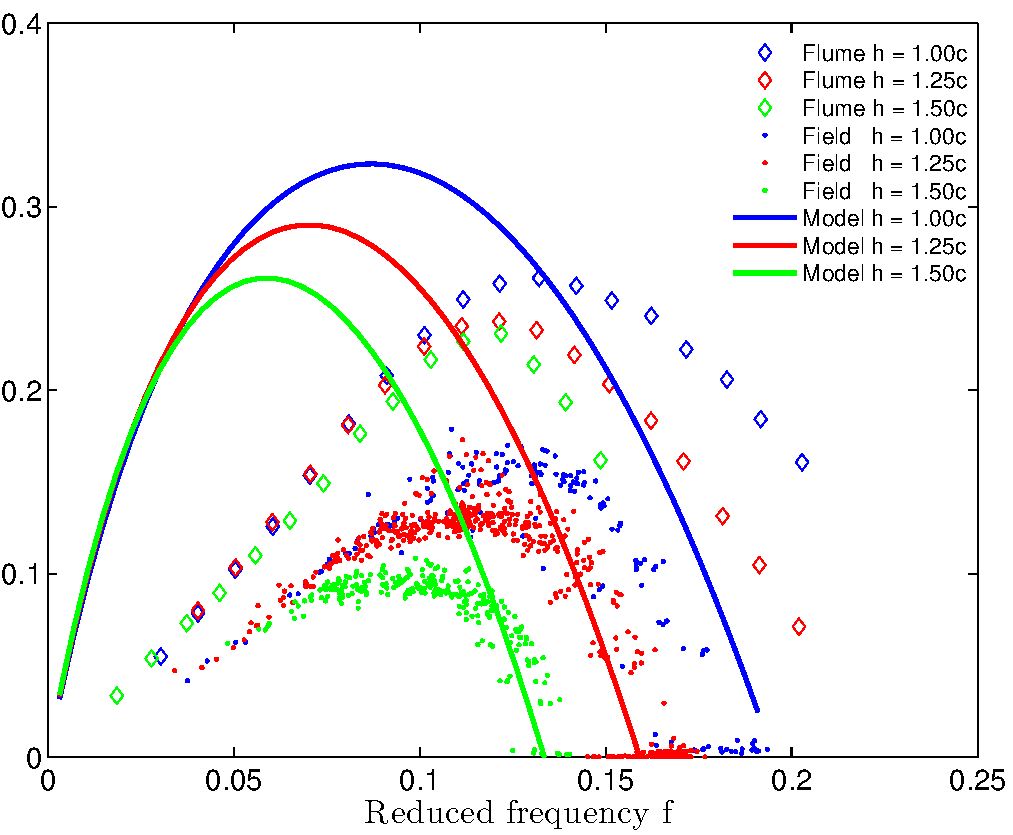
\includegraphics[width=12cm]{./Figures/theodorsen/Strouhal_vs_Efficiency.pdf} \\
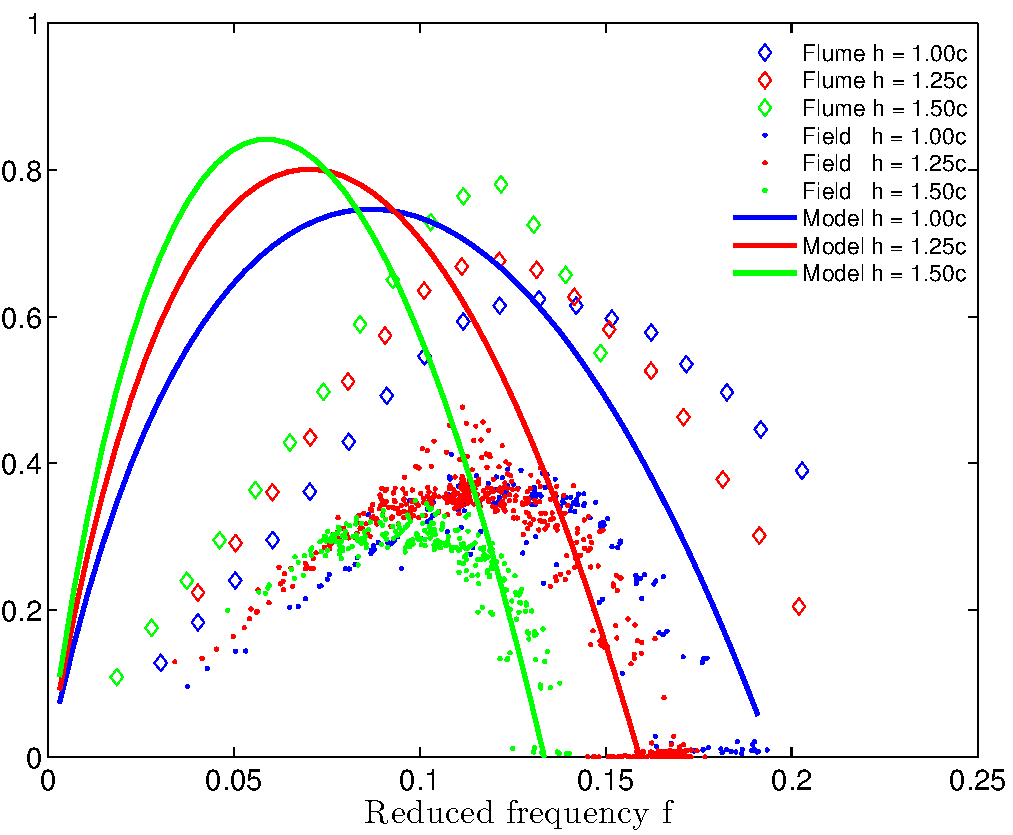
\includegraphics[width=12cm]{./Figures/theodorsen/Strouhal_vs_Cp.pdf}
\end{tabular}
\end{center}
\caption[The optimal energy efficiency for different stroke frequencies]{The dependence of energy efficiency on oscillating frequency for different heaving amplitude is shown with $\alpha = 70^o$, $\phi = 90^o$. }
\label{fig:Strouhal}
\end{figure}

What's more, this simple model of oscillating plate may shed some different light on the mechanism for the selection of optimal frequency for energy harvesting than those reported previously.
Zhu proposed that the flow energy extraction is closely related to the efficient evolution of the wake and particularly the optimal frequency is selected by the most unstable mode in the wake.
However, the simple model here, without any instabilities in the wake, also captures the optimal frequency pretty well.
On the other hand, both our model and the experimental data show that the optimal frequency is not quite sensitive to the heaving amplitude.
Zhu's DNS data shows exactly the same insensitivity and additionally the obviously different scenarios of instabilities in the wake for different heaving amplitudes, except that the energy efficiency with heaving amplitude close to the chord length is higher than the other cases.
 